%Copyright 2014 Jean-Philippe Eisenbarth
%This program is free software: you can 
%redistribute it and/or modify it under the terms of the GNU General Public 
%License as published by the Free Software Foundation, either version 3 of the 
%License, or (at your option) any later version.
%This program is distributed in the hope that it will be useful,but WITHOUT ANY 
%WARRANTY; without even the implied warranty of MERCHANTABILITY or FITNESS FOR A 
%PARTICULAR PURPOSE. See the GNU General Public License for more details.
%You should have received a copy of the GNU General Public License along with 
%this program.  If not, see <http://www.gnu.org/licenses/>.

%Based on the code of Yiannis Lazarides
%http://tex.stackexchange.com/questions/42602/software-requirements-specification-with-latex
%http://tex.stackexchange.com/users/963/yiannis-lazarides
%Also based on the template of Karl E. Wiegers
%http://www.se.rit.edu/~emad/teaching/slides/srs_template_sep14.pdf
%http://karlwiegers.com


\documentclass{scrreprt}

\usepackage{pdfpages}
\usepackage{listings}
\usepackage[T1]{fontenc}
\usepackage{placeins}
\usepackage{float}
\usepackage{underscore}
\usepackage[bookmarks=true]{hyperref}
\usepackage[utf8]{inputenc}
\usepackage{graphicx}
\usepackage{subfigure}
\usepackage[english]{babel}
\hypersetup{
	bookmarks=false,    % show bookmarks bar?
	pdftitle={Software Requirement Specification},    % title
	pdfauthor={Adam-Ryan},                     % author
	pdfsubject={TeX and LaTeX},                        % subject of the document
	pdfkeywords={TeX, LaTeX, graphics, images}, % list of keywords
	colorlinks=true,       % false: boxed links; true: colored links
	linkcolor=blue,       % color of internal links
	citecolor=black,       % color of links to bibliography
	filecolor=black,        % color of file links
	urlcolor=blue,        % color of external links
	linktoc=page            % only page is linked
}%
\def\myversion{1 }
\date{}
%\title
\usepackage{hyperref}
\begin{document}
	
	\begin{flushright}
		\rule{16cm}{5pt}\vskip1cm
		\begin{bfseries}
			\Huge{Tutorial 2\\}
			\vspace{1.9cm}
			for\\
			\vspace{1.9cm}
			Data Mining - Transformation
			\vspace{1.9cm}
			\LARGE{Version \myversion}\\
			\vspace{1.9cm}
			Adam Ryan (14395076)\\
			\vspace{1.9cm}
			COMP47530\\
			\vspace{1.9cm}
			\today\\
		\end{bfseries}
	\end{flushright}
	
	\tableofcontents

	
\chapter{Question 1}
\section{Exercise 1 - Questions}\label{E1Q}

A module coordinator has just completed the module assessments, and s/he would like to perform a quick analysis on the students results in various components of the module. The main objective is to see if there is any correlation between the assessment components. The students’ results are given in the file "Students\_Results.csv". Using Python script, answer the following questions:

\begin{enumerate}
\item Find the minimum, maximum, mean and standard deviation for each Homework column and the exam column
\item Add an additional named as ‘Homework Avg’ for the average homework mark for each student. Assume that the weighting of the homework average is 25\% and that of the examination is 75\%, add an additional column named 'Overall Mark' for the overall folded mark.
\item  Construct a correlation matrix of homework and exam variables. What can you conclude from the matrix?
\item Discuss various ways of treating the missing values in the dataset.
\item Use UCD grading system to convert the final mark into a grade (column named ‘Grade’). Produce a histogram for the grades.
\item Save the newly generated dataset to "./output/question1\_out.csv".
\end{enumerate}

	
\section{Question 1 - Answer}
This is the answer to question one on the tutorial sheet. 

\begin{enumerate}
	\item Find the minimum, maximum, mean and standard deviation for each Homework column and the exam column
\begin{itemize}
\item For the beginning step, we observe there are 54 rows of data. In total, one student has Homework 1 not completed, no students have not completed homework 2, and 6 students have not completed Homework 3. As the context of the question is in relation to assessment, we can assume that homeworks without grades were homeworks which were not submitted. Therefore, as an initial data cleansing exercise, we replace missing values with 0.
\item Of the students who did complete the homeworks (i.e. of students with data populated) the stats are:
\begin{itemize}
	\item Homework 1 \begin{itemize}
		\item Minimum: 31
		\item Maximum: 90
		\item Standard Deviation: 17.877782
		\item Mean: 55.641509
	\end{itemize}
	\item Homework 2
\begin{itemize}
	\item Minimum: 0
	\item Maximum: 98
	\item Standard Deviation: 15.441612	
	\item Mean: 89.83...
\end{itemize}
	\item Homework 3
\begin{itemize}
	\item Minimum: 5
	\item Maximum: 100
	\item Standard Deviation: 21.585216	
	\item Mean: 47.687500
\end{itemize}
\end{itemize}

\item After fixing the data quality error described above by replacing all missing values with 0 due to the context, we calculate the values as:
\begin{itemize}
	\item Homework 1 \begin{itemize}
\item Minimum: 0.0
\item Maximum: 90.0
\item Mean: 54.611111111111114
\item Std. Deviation: 19.259319397315124
	\end{itemize}
	\item Homework 2
	\begin{itemize}
  \item Minimum: 0.0
\item Maximum: 98.0
\item Mean: 89.83333333333333
\item  Std. Deviation: 15.441612487898249
Count: 54.0
	\end{itemize}
	\item Homework 3
	\begin{itemize}
\item Minimum: 0.0
\item Maximum: 100.0
\item Mean: 42.388888888888886
\item Std. Deviation: 25.338029190733053
	\end{itemize}

\item I use the dataframe describe feature which is present in pandas and provides descriptive statistics for numerical columns as this process is quick and the volume of data small enough to allow pandas usage.
\end{itemize}
\end{itemize}
\item Add an additional named as ‘Homework Avg’ for the average homework mark for each student. Assume that the weighting of the homework average is 25\% and that of the examination is 75\%, add an additional column named 'Overall Mark' for the overall folded mark.

\begin{itemize}
	\item I continue using the cleansed dataset as described in the previous question, where missing Homework values were replaced by zero, cleanse the exam column in the same method (as this has one missing value), and add on the described column using pandas.
\end{itemize}

\item  Construct a correlation matrix of homework and exam variables. What can you conclude from the matrix?
\begin{itemize}
	\item  I use the correlation method on dataframe to produce the matrix. We see that the homeworks are, in general, only weakly positively correlated with one another. The first homework's grade is much more strongly correlated with the exam results (with a value of 0.6 rounded to one decimal place) compared to the other homeworks. However, while Homework 1 was more strongly correlated with the exam results, the other two homeworks were more strongly correlated with the homework average. This homework average is elevated by the overall strong performance of students on the second homework which, as we see from the descriptive statistics, are highly inflated compared to Homework 1 and Homework 3. The correlation matrix, again after cleansing the missing values, is below:
	\begin{figure}[h]
		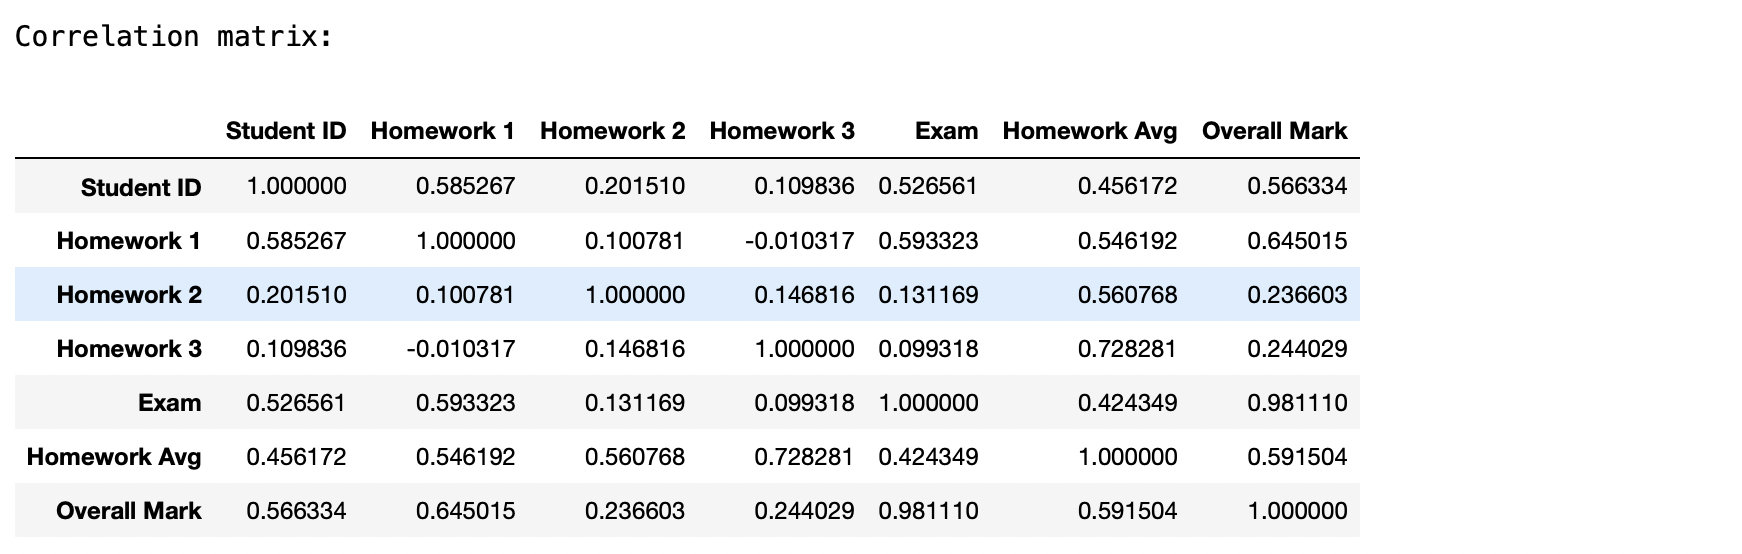
\includegraphics[width=12cm]{DM_Corr.png}
		\centering
	\end{figure}
\item I do not remove the student ID (from the photo above) in creating the correlation matrix as this can be ignored in interpretting the result as the first row and column in the set, but it can be seen that this is removed in the submission file.
\end{itemize}

\item Discuss various ways of treating the missing values in the dataset.
\begin{itemize}
	\item As described in the tutorial, we were instructed to cleanse the homework and exam columns prior to calculations in question 1. \item The first method of cleansing, which I implemented, is to populate the missing values with 0. This method is sensible in the context of homework assignments and exams, as students may have not completed the assignment or exam in which case they should receive a zero. 
	\item The second method is to leave these data as empty; students may have received extenuating circumstances resulting in these components not being weighted for grading or no homework grade being assigned. In this instance, a null value is more sensible for the assignment than any numerical grade as it's a more accurate description of the grade (i.e. it is not applicable). 
	\item Another method to cleanse the data would be to assign the class average to the homework or exam columns. This method is not sensible given the context, as it punishes students who received below the mean grade who submitted the assignments while rewarding those who did not complete the assignment.
\end{itemize}

\item Use UCD grading system to convert the final mark into a grade (column named ‘Grade’). Produce a histogram for the grades.
\begin{itemize}
\item A histogram looks at numeric values rather than the categorical grades, so I have produced a barplot of the grades and a histogram of the marks as displayed below. We see the grades are concentrated around a C grade, and skews leans towards higher marks as opposed to being more evenly distributed across all grades:

\begin{figure}[!h]
	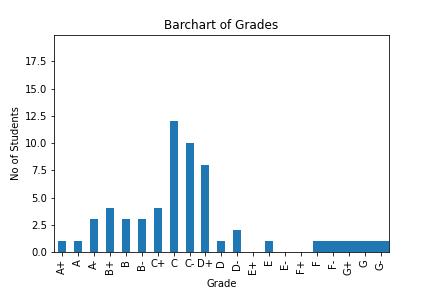
\includegraphics[width=8cm]{barchart_of_grades_q1.png}
	\centering
\end{figure}

\begin{figure}[!h]
		\centering
	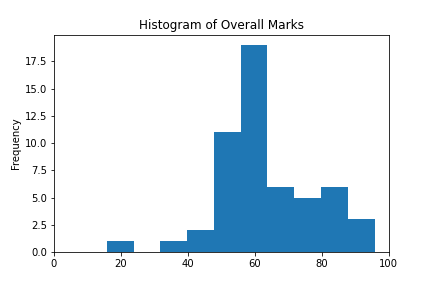
\includegraphics[page=1, width=0.95\linewidth]{histogram_of_grades_q1.png}
	\centering
\end{figure}
\end{itemize}

\item Save the newly generated dataset to "./output/question1\_out.csv".
\begin{itemize}
	\item Done.
\end{itemize}
\end{enumerate}

Please note that in the test script, there are roundings of grades which occur; in order to pass the test script I have had to adjust some calculations to round however I would not ordinarily this. Similarly, there is a customer which is flaged as being an A grade when with the computer science conversion grading scheme they are actually an A-. In my grade bucketing, I have explicilty used the Computer Science grading scheme rather than the general UCD grading scheme. 

\newpage
\chapter{Question 2}
\section{Exercise 2 - Questions}\label{E2Q}

The file "Sensor\_Data.csv" contains data obtained from a sensory system. Some of the
attributes in the file need to be normalised, but you don't want to lose the original values.


\begin{enumerate}
	\item Generate a new attribute called "Original Input3" which is a copy of the attribute "Input3". Do the same with the attribute "Input12" and copy it into Original "Input12".
	\item Normalise the attribute "Input3" using the z-score transformation method.
	\item Normalise the attribute "Input12" in the range [0:0; 1:0].
	\item Generate a new attribute called "Average Input", which is the average of all the attributes
	from "Input1" to "Input12". This average should include the normalised attributes values but not the copies that were made of these.
	\item Save the newly generated dataset to "./output/question2\_out.csv".
\end{enumerate}



\section{Exercise 2 - Answers}
This is solution to the question in Exercise 2. 


\begin{enumerate}
	\item Generate a new attribute called "Original Input3" which is a copy of the attribute "Input3". Do the same with the attribute "Input12" and copy it into Original "Input12".
	\begin{itemize}
		\item Done.
	\end{itemize}
	\item Normalise the attribute "Input3" using the z-score transformation method.
	\begin{itemize}
		\item Done, wrote the method.
	\end{itemize}
	
	\item Normalise the attribute "Input12" in the range \[ 0:0; 1:0\].
	\begin{itemize}
		\item Done, wrote the method.
	\end{itemize}
	
	\item Generate a new attribute called "Average Input", which is the average of all the attributes
	from "Input1" to "Input12". This average should include the normalised attributes values but not the copies that were made of these.
	\begin{itemize}
		\item Done, mean over list of columns in df with format of column name as 'input' and number less than thirteen with axis of one.
	\end{itemize}
	
	\item Save the newly generated dataset to "./output/question2\_out.csv".
	\begin{itemize}
		\item Done
	\end{itemize}
	
\end{enumerate}

\newpage	
\chapter{Question 3}
\section{Exercise 3 - Questions}
The files "DNA\_Data.csv" contains biological data arranged into multiple columns. We need to compress the information contained in the data.
\begin{enumerate}
\item Reduce the number of attributes using Principal Component Analysis (PCA), making sure at least 95\% of all the variance is explained.
\item Discretise the PCA-generated attribute subset into 10 bins, using bins of equal width. For each component X that you discretise, generate a new column in the original dataset named "pcaX\_width". For example, the first discretised principal component will correspond to a new column called "pca1\_width".
\item Discretise PCA-generated attribute subset into 10 bins, using bins of equal frequency (they should all the same number of points). For each component X that you discretise, generate a new column in the original dataset named "pcaX\_freq". For example, the first discretised principal component will correspond to a new column called "pca1\_freq".
\item Save the generated dataset to "./output/question3\_out.csv".
\end{enumerate}




\section{Exercise 3 - Answers}	
The following are the answers to exercise 3 in the first tutorial sheet:

\begin{enumerate}
	\item Reduce the number of attributes using Principal Component Analysis (PCA), making sure at least 95\% of all the variance is explained.
	\begin{itemize}
		\item This is complete. I wrote a script which adds components until the cumulative amount reaches a cut off and then returns that data. I used SKLearn to do this.
	\end{itemize}
	\item Discretise the PCA-generated attribute subset into 10 bins, using bins of equal width. For each component X that you discretise, generate a new column in the original dataset named "pcaX\_width". For example, the first discretised principal component will correspond to a new column called "pca1\_width".
		\begin{itemize}
		\item Pandas contains a function qcut and cut to achieve this, and I implemented a method that loops over all PCA columns and adds on the width and frequency using cut and qcut with the desired number of bins.
	\end{itemize}
	\item Discretise PCA-generated attribute subset into 10 bins, using bins of equal frequency (they should all the same number of points). For each component X that you discretise, generate a new column in the original dataset named "pcaX\_freq". For example, the first discretised principal component will correspond to a new column called "pca1\_freq".
		\begin{itemize}
		\item Pandas contains a function qcut and cut to achieve this, and I implemented a method that loops over all PCA columns and adds on the width and frequency using cut and qcut with the desired number of bins.
	\end{itemize}
	\item Save the generated dataset to "./output/question3\_out.csv".
		\begin{itemize}
		\item Done
	\end{itemize}
	
\end{enumerate}

	
\end{document}
